\chapter{Mechanizmy współbieżności oferowane przez Project Loom}

Trzeci rozdział pracy poświęcony jest omówieniu najważniejszych mechanizmów dostępnych w ramach Project Loom -- inicjatywy usprawniającej tworzenie aplikacji współbieżnych w środowisku JVM. Rozdział zawiera zwięzłą prezentację historii powstawania tego projektu, a także omówienie najważniejszych mechanizmów, które on oferuje, tj. odrębną kategorię wątków, określanych mianem wątków wirtualnych (ang. \emph{virtual threads}), mechanizm współbieżności strukturalnej (ang.~~\emph{structured concurrency}) i~mechanizm przekazywania danych kontekstowych w~ramach zmiennych zakresowych (ang. \emph{scoped values}).
% Rozdział zawiera również omówienie technik integracji mechanizmów oferowanych przez Project Loom z~istniejącymi w~środowisku JVM modelami współbieżności.

\section{Wprowadzenie do Project Loom}

Project Loom jest inicjatywą zapoczątkowaną pod koniec 2017 roku przez OpenJDK. W ramach projektu wyróżnia się trzy główne składowe:
\begin{itemize}
    \item mechanizm \emph{wirtualnych wątków} (ang. \emph{virtual threads}), będący alternatywą dla klasycznego mechanizmu wątków (wątków platformowych) i zdefiniowany w~dokumencie JEP\footnote{JEP (\emph{JDK Enhancement Proposal}) to formalny dokument opisujący proponowane zmiany, nowe funkcjonalności lub usprawnienia platformy JDK.} o numerze 444 \cite{jep444},
    \item mechanizm \emph{współbieżności strukturalnej} (ang. \emph{structured concurrency}), umożliwiający uporządkowanie pracy z wątkami poprzez dodanie tak zwanych \emph{zakresów zadań} (ang. \emph{task scopes}) i strategii zachowań w przypadku wystąpienia błędu lub przerwania działania wątku, opisany w dokumencie JEP~525 \footnote{W chwili publikacji najnowsza wersja mechanizmu współbieżności strukturalnej została udostępniona w wersji \textit{preview}, co oznacza, że jest dostępna w standardowym JDK, lecz jej składnia lub semantyka mogą ulec zmianie przed ostatecznym włączeniem do specyfikacji platformy Java.} \cite{jep525},
    \item mechanizm przekazywania danych kontekstowych między wątkami za pomocą \emph{zmiennych zakresowych} (ang. \emph{scoped values}), będący alternatywą dla klasy \texttt{ThreadLocal} w systemach współbieżnych i opisany w dokumencie JEP~506 \cite{jep506}.
\end{itemize}

Początkowo, ideą projektu było wprowadzenie lekkich wątków użytkownika (ang. \emph{user-mode threads}) oraz uproszczenie programowania współbieżnego, szczególnie w~aplikacjach, których dużą częścią są blokujące zadania, takich jak serwery i~systemy sieciowe \cite{openjdk-loom-proposal}. Wraz z upływem czasu zakres projektu został rozszerzony o mechanizmy zwiększające bezpieczeństwo aplikacji współbieżnych i ustrukturyzowanie pracy z wątkami. Project Loom wciąż ewoluuje, głównie w kontekście zmian w API poszczególnych mechanizmów, lecz większość z nich jest integralną częścią JDK, dodanych w ramach oficjalnych wydań.

\section{Wirtualne wątki (\emph{Virtual Threads})}

Mechanizm wirtualnych wątków, we wczesnych fazach projektu określanych mianem \emph{fibers} \cite{openjdk-loom-proposal}, to chronologicznie pierwsza z trzech głównych składowych projektu Loom, która pod tą nazwą po raz pierwszy pojawiła się w JDK w wersji 19 w~ramach wersji poglądowej (ang. \emph{preview}), a została oficjalnie wydana w ramach JDK 21. Mechanizm ten jest alternatywą dla wątków platformowych, opisanych w~sekcji \hyperref[sec:thread-api]{2.3.1 Klasyczny model współbieżności (Thread API)}.

W celu wyjaśnienia potrzeby wprowadzenia mechanizmu wirtualnych wątków do środowiska JVM, dokument \textit{JEP 444: Virtual Threads} \cite{jep444} powołuje się na prawo Little’a, które wiąże ze sobą latencję, współbieżność i przepustowość w kontekście skalowalności aplikacji współbieżnych:

\begin{displayquote}
    \textit{Dla danego czasu przetwarzania żądania (tj. latencji) liczba żądań obsługiwanych jednocześnie przez aplikację (tj. współbieżność) musi rosnąć proporcjonalnie do tempa napływu żądań (tj. przepustowości).}
\end{displayquote}

\noindent
Jak wspomniano w sekcji \hyperref[sec:thread-api]{2.3.1 Klasyczny model współbieżności (Thread API)}, wątki platformowe w środowisku JVM są zaimplementowane jako obiekty opakowujące (ang. \emph{wrappers}) wątki systemu operacyjnego. Wątki te są zasobożerne, co uniemożliwia ich tworzenie w bardzo dużych ilościach, przez co liczba wątków często staje się czynnikiem ograniczającym skalowalność, na długo przed wyczerpaniem innych zasobów.

Próbą rozwiązania problemu zasobożerności wątków platformowych jest zastosowanie podejścia opartego na współdzieleniu wątków i programowaniu asynchronicznym (patrz sekcja \hyperref[sec:reactive]{2.3.3 Reaktywny model współbieżności (Reactive Streams, Project Reactor, RxJava)}), które umożliwia obsługę dużej liczby współbieżnych operacji przy ograniczonej liczbie wątków systemowych. Rozwiązanie to eliminuje problem kosztowności wątków systemu operacyjnego, jednak odbywa się kosztem znacznego wzrostu złożoności programowania. Asynchroniczny styl wymusza dekompozycję logiki aplikacyjnej na etapy realizowane w postaci wyrażeń lambda, co uniemożliwia wykorzystanie modelu współbieżności obecnego do tej pory w środowisku JVM.

Wirtualne wątki umożliwiają zachowanie paradygmatu \emph{thread-per-request}\footnote{Paradygmat \emph{thread-per-request} zakłada, że każde przychodzące żądanie jest obsługiwane przez dedykowany wątek.} przy jednoczesnym osiągnięciu skalowalności porównywalnej z podejściem asynchronicznym.
% jeszcze parę zdań o tym

\subsubsection{Cykl życia wirtualnych wątków}
% opisac schemat virtual threads <-> carrier threads <-> OS threads
% opisac fakt ze nie warto tworzyć puli VT

Każdorazowo, gdy tworzony jest wirtualny wątek, zostaje on dodany do \emph{kolejki wirtualnych wątków}, będącą kolejką typu FIFO (ang. \emph{First In, First Out}). Wirtualny wątek może wykonać przydzielone mu zadanie, gdy zostanie przypisany do \emph{wątku nośnego} (ang. \emph{carrier thread}). Reprezentuje on wątek platformowy (tj.~wątek systemu operacyjnego) po stronie platformy JVM \cite{veen2024}. Każdy wątek nośny ma przypisany odpowiadający mu wątek platformowy i domyślnie ich liczba jest równa liczbie dostępnych (fizycznych) procesorów logicznych \cite{openjdk-vt-presentation}. W odróżnieniu od~wątków platformowych i nośnych, liczba wirtualnych wątków nie jest zależna od~liczby dostępnych procesorów logicznych, a w większości przypadków ją przekracza. Wynika to ze sposobu zarządzania cyklem ich życia, który został przedstawiony na rysunku \ref{fig:vt-lifecycle}.

\begin{figure}[ht]
    \centering
    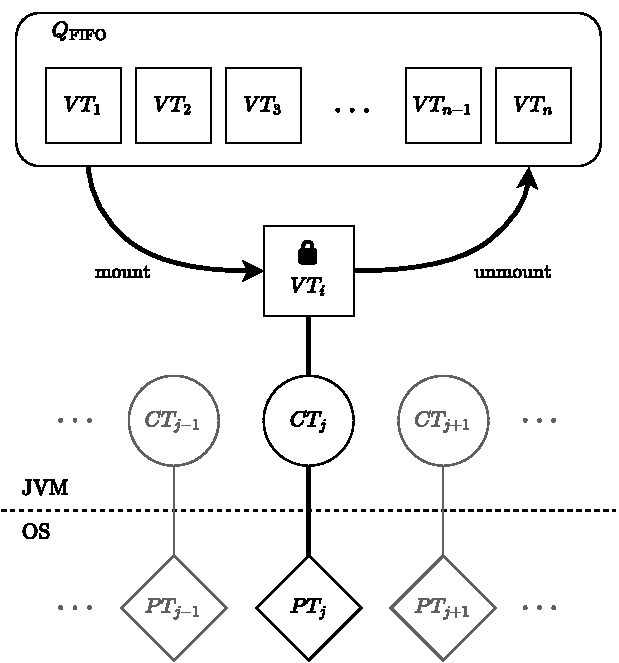
\includegraphics[width=0.75\textwidth]{rozdzialy/rozdzial3/img/VT-lifecycle.pdf}
    \caption{Cykl życia wirtualnych wątków w środowisku JVM}
    \source{opracowanie własne na podstawie \cite{veen2024}}
    \label{fig:vt-lifecycle}
\end{figure}

Korzystając z oznaczeń zawartych na rysunku \ref{fig:vt-lifecycle}, cykl życia wirtualnych wątków w środowisku JVM w kontekście jednego wątku nośnego można opisać następująco:
\begin{enumerate}
    \item Każdy nowy wirtualny wątek $VT$ zostaje dodany na koniec kolejki wirtualnych wątków $Q_{\mathrm{FIFO}}$
    \item Planista (ang. \emph{scheduler}) wątków wirtualnych, obecny w środowisku JVM, bierze pierwszy wolny wątek wirtualny z kolejki przypisuje go (ang. \emph{mount}) do wolnego wątku nośnego ($CT_j$)
    \item Wątek nośny $CT_j$, odpowiadający wątkowi platfomowemu $PT_j$, wykonuje kod przypisany do przydzielonego mu wątku wirtualnego $VT_i$
    \item Gdy wątek wirtualny $VT_i$ wykonuje operację blokującą (stan reprezentowany przez symbol kłódki \faLock), JVM zapisuje jego aktualny stan, dodaje go na koniec kolejki $Q_{\mathrm{FIFO}}$, jednocześnie zwalniając (ang. \emph{unmount}) wątek nośny $CT_j$
    \item JVM przypisuje kolejny wątek wirtualny (tj. pierwszy w kolejce $Q_{\mathrm{FIFO}}$) do wątku nośnego $CT_j$
\end{enumerate}

\section{Współbieżność strukturalna (\emph{Structured Concurrency})}
% doczytać JEP-y
% opisać różnicę: unstructured concurrency vs structured concurrency
% opisać strukturę i działanie StructuredTaskScope

\section{Zmienne zakresowe (\emph{Scoped Values})}
% przeczytać JEP-a

% \section{Integracja mechanizmów Project Loom z~istniejącymi modelami współbieżności}